\documentclass{beamer}

\usepackage{float}
\usepackage{subfig}
\usepackage{graphicx}
\graphicspath{{../figures/}}

%Information to be included in the title page:
\title{Exploration of Abalone game-playing agents}
\author{Ture Claussen}
\date{2021-06-14}


\begin{document}

\frame{\titlepage}

\begin{frame}
	\begin{figure}
		\frametitle{Rules}
		\centering
		\subfloat[Starting position]{
			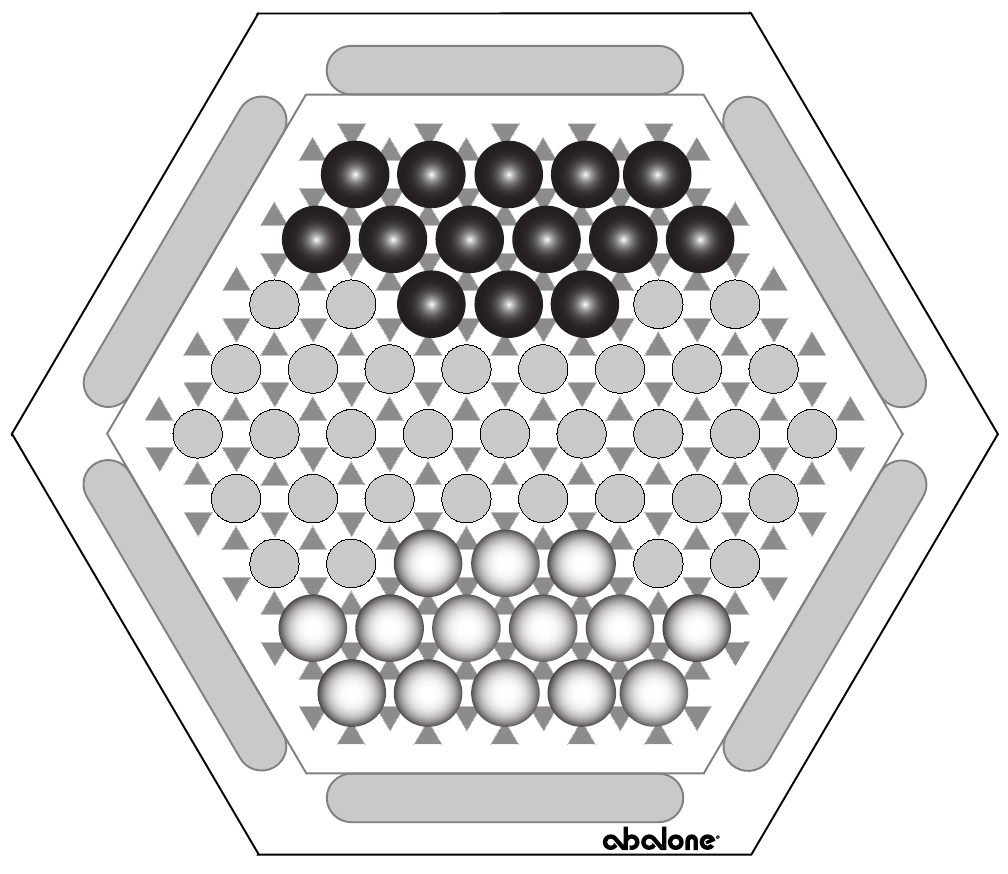
\includegraphics[width=3cm, keepaspectratio]{rules_starting_position.png}
		}
		\hfill
		\subfloat["In-line" moves]{
			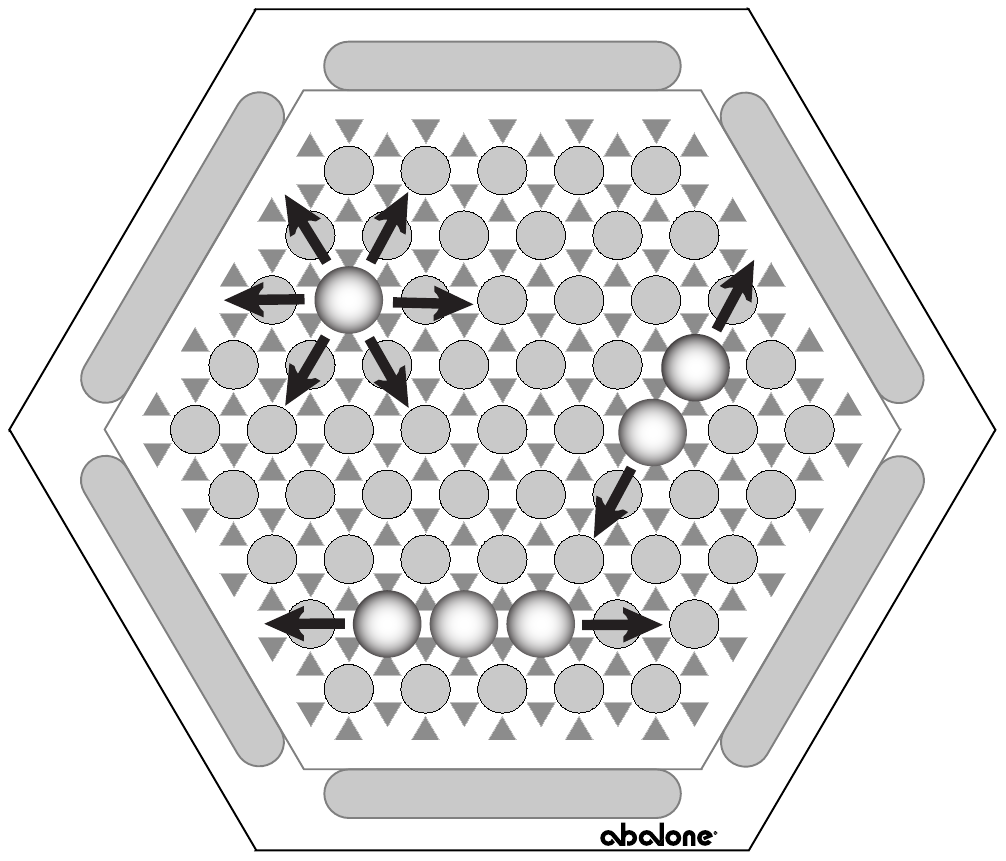
\includegraphics[width=3cm, keepaspectratio]{rules_inline_move.png}
		}
		\hfill
		\subfloat["Side-step" moves]{
			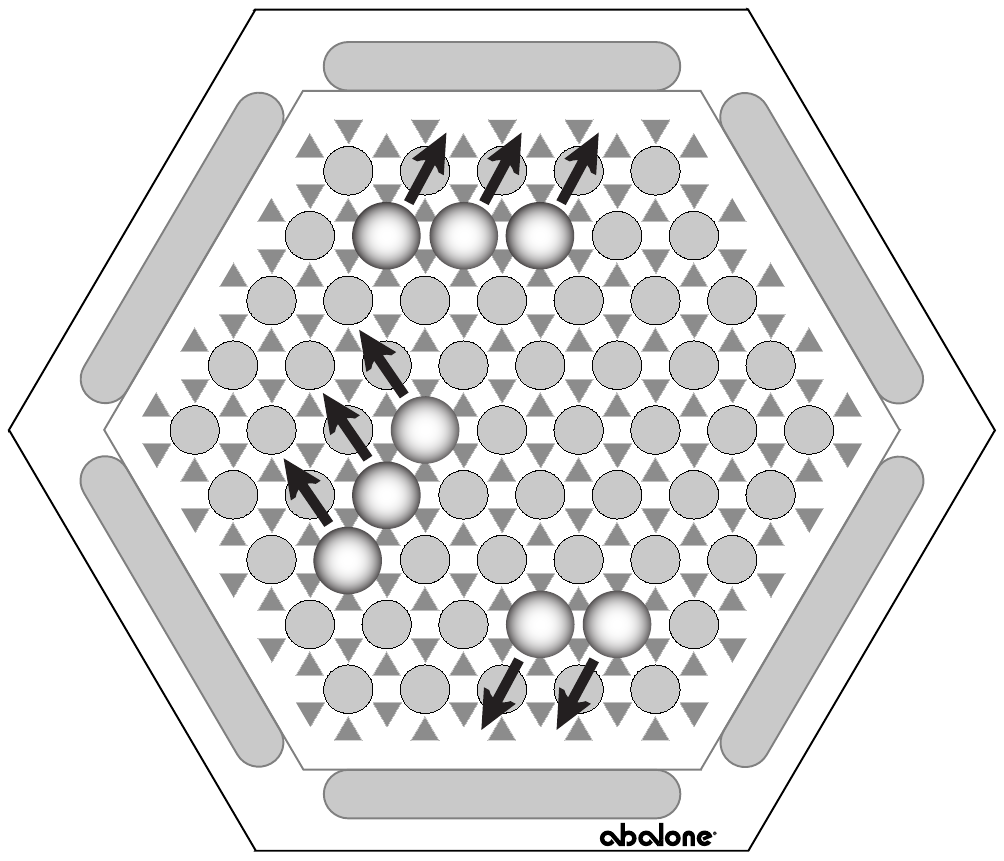
\includegraphics[width=3cm, keepaspectratio]{rules_side_step_move.png}
		}
	\end{figure}
\end{frame}

\begin{frame}

	\frametitle{Agent design: PEAS}

	\begin{description}
		\item[Performance measure] Win/loss, number of moves, time to deliberate
		\item[Environment] Digital playing board
		\item[Actuators] Move marbles, display text to CLI
		\item[Sensors] Position of marbles
	\end{description}
\end{frame}
\begin{frame}

	\frametitle{Agent design: Environment}

	\begin{itemize}
		\item fully observable
		\item two-agent
		\item competitive
		\item sequential
		\item static and discrete
	\end{itemize}
\end{frame}

\begin{frame}
	\frametitle{State space complexity}

	$$
		\sum_{k=8}^{14}\sum_{m=9}^{14}\frac{61!}{k!(61-k)!}\times\frac{(61-k)!}{m!((61-k)-m)!}
	$$
\end{frame}
\begin{frame}
	\frametitle{Game tree complexity}
	\begin{itemize}
		\item Average branching factor $b$ of 60
		\item Average length of game $d$ of 87 \cite{lemmens_constructing_2005}
	\end{itemize}
	$$ b^d = 60^{87}$$

	\begin{figure}
		\centering
		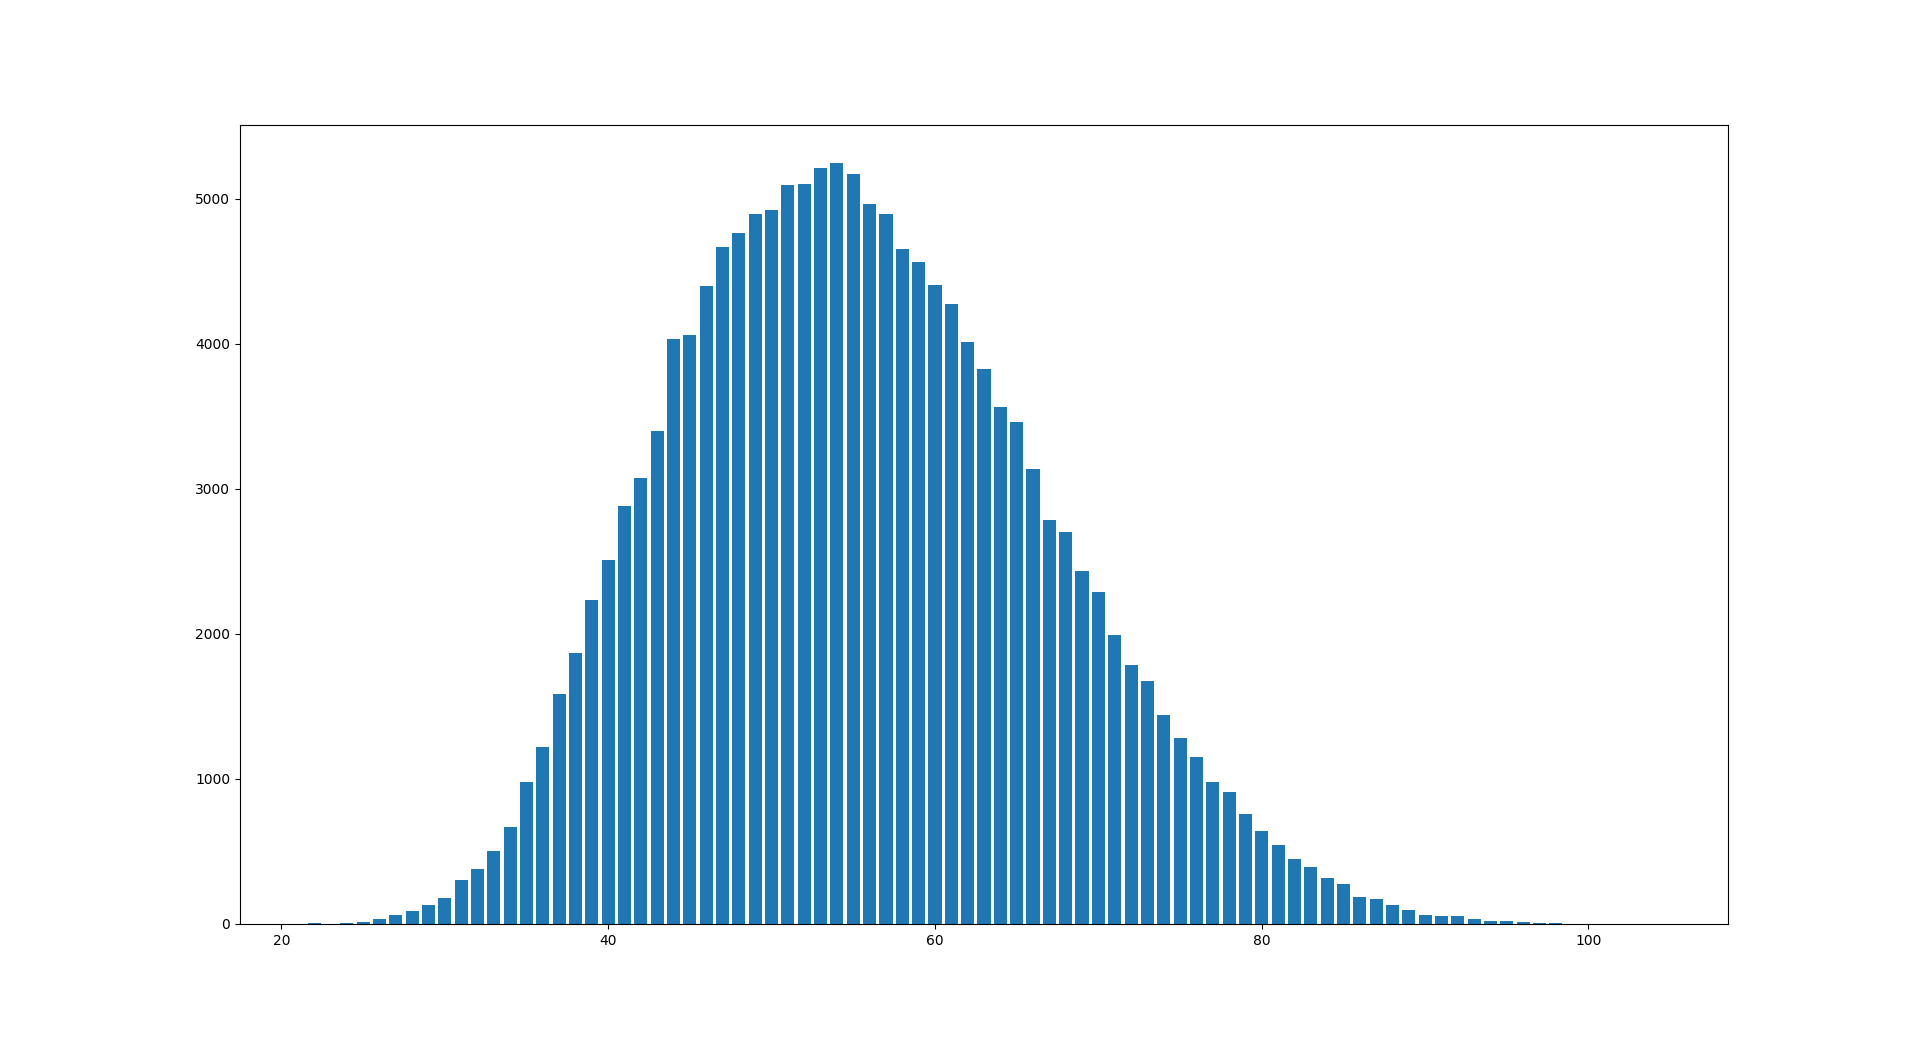
\includegraphics[width=7cm, keepaspectratio]{distribution_of_moves.png}
		\caption{Counts of moves available for random for random player in 5 games}
	\end{figure}
\end{frame}

\begin{frame}
	\frametitle{Complexity Comparision}
	\centering
	\begin{tabular}{ | c | c | c | }
		\hline
		Game        & \small{state-space complexity (log)} & \small{game-tree complexity} (log) \\
		\hline
		Tic-tac-toe & 3                                    & 5                                  \\
		\hline
		Reversi     & 28                                   & 58                                 \\
		\hline
		Chess       & 46                                   & 123                                \\
		\hline
		Abalone     & 24                                   & 154                                \\
		\hline
		Go          & 172                                  & 360                                \\
		\hline
	\end{tabular}
\end{frame}

\end{document}
